\documentclass[10pt]{article}
\usepackage[letterpaper]{geometry}
\geometry{verbose,tmargin=1in,bmargin=1in,lmargin=1in,rmargin=1in}
\usepackage{setspace}
\usepackage{ragged2e}
\usepackage{color}
\usepackage{titlesec}
\usepackage{graphicx}
\usepackage{float}
\usepackage{mathtools}
\usepackage{amsmath}
\usepackage[font=small,labelfont=bf,labelsep=period]{caption}
\usepackage[english]{babel}
\usepackage{indentfirst}
\usepackage{array}
\usepackage{makecell}
\usepackage[usenames,dvipsnames]{xcolor}
\usepackage{multirow}
\usepackage{tabularx}
\usepackage{arydshln}
\usepackage{caption}
\usepackage{subcaption}
\usepackage{xfrac}
\usepackage{etoolbox}
\usepackage{cite}
\usepackage{url}
\usepackage{dcolumn}
\usepackage{hyperref}
\usepackage{courier}
\usepackage{url}
\usepackage{esvect}
\usepackage{commath}
\usepackage{verbatim} % for block comments
\usepackage{enumitem}
\usepackage{hyperref} % for clickable table of contents
\usepackage{braket}
\usepackage{titlesec}
\usepackage{booktabs}
\usepackage{gensymb}
\usepackage{longtable}
\usepackage{listings}
\usepackage{cancel}
\usepackage{tcolorbox}
\usepackage[mathscr]{euscript}
\lstset{
    frame=single,
    breaklines=true,
    postbreak=\raisebox{0ex}[0ex][0ex]{\ensuremath{\color{red}\hookrightarrow\space}}
}

% for circled numbers
\usepackage{tikz}
\newcommand*\circled[1]{\tikz[baseline=(char.base)]{
            \node[shape=circle,draw,inner sep=2pt] (char) {#1};}}


\titleclass{\subsubsubsection}{straight}[\subsection]

% define new command for triple sub sections
\newcounter{subsubsubsection}[subsubsection]
\renewcommand\thesubsubsubsection{\thesubsubsection.\arabic{subsubsubsection}}
\renewcommand\theparagraph{\thesubsubsubsection.\arabic{paragraph}} % optional; useful if paragraphs are to be numbered

\titleformat{\subsubsubsection}
  {\normalfont\normalsize\bfseries}{\thesubsubsubsection}{1em}{}
\titlespacing*{\subsubsubsection}
{0pt}{3.25ex plus 1ex minus .2ex}{1.5ex plus .2ex}

\makeatletter
\renewcommand\paragraph{\@startsection{paragraph}{5}{\z@}%
  {3.25ex \@plus1ex \@minus.2ex}%
  {-1em}%
  {\normalfont\normalsize\bfseries}}
\renewcommand\subparagraph{\@startsection{subparagraph}{6}{\parindent}%
  {3.25ex \@plus1ex \@minus .2ex}%
  {-1em}%
  {\normalfont\normalsize\bfseries}}
\def\toclevel@subsubsubsection{4}
\def\toclevel@paragraph{5}
\def\toclevel@paragraph{6}
\def\l@subsubsubsection{\@dottedtocline{4}{7em}{4em}}
\def\l@paragraph{\@dottedtocline{5}{10em}{5em}}
\def\l@subparagraph{\@dottedtocline{6}{14em}{6em}}
\makeatother

\newcommand{\volume}{\mathop{\ooalign{\hfil$V$\hfil\cr\kern0.08em--\hfil\cr}}\nolimits}

\setcounter{secnumdepth}{4}
\setcounter{tocdepth}{4}
\begin{document}

\title{ME 280a: HW 6}
\author{April Novak}

\maketitle

\section{Introduction and Objectives}

The purpose of this study is to construct the Finite Element (FE) problem statement for a 2-D heat conduction problem, and then to solve said problem on a relatively complex domain.

\section{Procedure}
\label{sec:Procedure}

This section details the problem statement and mathematical method used for solving the problem.

\subsection{The Analytical Solution}

This problem solves the heat conduction problem, with a governing equation given by:

\begin{equation}
\nabla\cdot(k\nabla T)+f=0
\end{equation}

where \(k\) is the thermal conductivity, \(T\) the temperature (scalar), and \(f\) a volumetric heat source/sink. This problem is to be solved with two different sets of specifications. For one of these sets, there is an analytical solution to offer a comparison to ensure that the code functions correctly, and for the second, there is no analytical solution. Both specifications have the following boundary conditions:

\begin{equation}
\begin{aligned}
T(\theta=\pi)=T_0\\
-k\nabla T\cdot\hat{n}|_{\theta=0}=q_o(r)\\
-k\nabla T\cdot\hat{n}|_{\theta\neq0\cup \theta\neq\pi}=0\\
\end{aligned}
\end{equation}

For the analytical solution, these specifications are:

\begin{equation}
\label{eq:AnalyticalSpecs}
\begin{aligned}
T_o=110\\
q_o(r)=\frac{20}{r}\\
f(r,\theta)=\frac{40}{r^2}\sin{(2\theta)}\\
\end{aligned}
\end{equation}

To obtain the analytical solution, the governing equation is written explicitly in polar coordinates:

\begin{equation}
\frac{1}{r}\frac{\partial}{\partial r}\left(kr\frac{\partial T}{\partial r}\right)+\frac{1}{r^2}\frac{\partial}{\partial\theta}\left(k\frac{\partial T}{\partial\theta}\right)+\frac{40}{r^2}\sin{(2\theta)}=0
\end{equation}

where \(f(r,\theta)\) has been inserted from Eq. \eqref{eq:AnalyticalSpecs}. Because \(k\) is constant with these specifications, it can be moved outside the derivatives. Because boundary conditions are only asymmetric in the \(\theta\) direction (i.e. boundary conditions are insulated on the \(r\)-sides of the tube), the solution is not a function of \(r\). 

\begin{equation}
k\frac{\partial}{\partial\theta}\left(\frac{\partial T}{\partial\theta}\right)+40\sin{(2\theta)}=0
\end{equation}

Rearranging, and integrating once in \(\theta\):

\begin{equation}
d\left(\frac{d T}{d\theta}\right)=-\frac{40}{k}\sin{(2\theta)}d\theta\quad\rightarrow\quad \frac{dT}{d\theta}=\frac{20}{k}\cos{(2\theta)}+C_o
\end{equation}

Integrating once more:

\begin{equation}
T(\theta)=\frac{10}{k}\sin{(2\theta)}+C_o\theta+C_1
\end{equation}

where \(C_o\) and \(C_1\) are constants of integration. These constants are determined by applying the boundary conditions:

\begin{equation}
T(\pi)=T_o=C_o\pi+C_1
\end{equation}

\begin{equation}
-k\frac{1}{r}\frac{dT(\theta=0)}{d\theta}=-k\frac{1}{r}\left(\frac{20}{k}+C_o\right)=\frac{20}{r}
\end{equation}

These equations give:

\begin{equation}
\begin{aligned}
C_1=T_o-\frac{40}{k}\pi\\
C_o=\frac{40}{k}\\
\end{aligned}
\end{equation}




\subsection{The Weak Form}

The weak form is obtained by multiplying through by a test function \(\psi\) and integrating over the body:

\begin{equation}
\label{eq:StrongForm2}
\int_{\Omega}\nabla\cdot(k\nabla T)\psi d\Omega=-\int_{\Omega}f\psi d\Omega
\end{equation}

Applying the product rule in Eq. \eqref{eq:StrongForm2}:

\begin{equation}
\begin{aligned}
-\int_{\Omega}k\nabla T\nabla\psi d\Omega+\int_{\partial\Omega}k\nabla T\psi\cdot\hat{n}dA=-\int_{\Omega}f\psi d\Omega\\
\int_{\Omega}k\nabla T\nabla\psi d\Omega=\int_{\Omega}f\psi d\Omega+\int_{\partial\Omega}k\nabla T\psi\cdot\hat{n}dA\\
\end{aligned}
\end{equation}

Because the shape functions are defined to be zero on Dirichlet boundaries, the above area integral can be specified as the boundaries over which there are flux boundary conditions:

\begin{equation}
\int_{\Omega}k\nabla T\nabla\psi d\Omega=\int_{\Omega}f\psi d\Omega+\int_{\Gamma_q}\textbf{q}^{*}\psi dA\\
\end{equation}

where \(\Gamma_q\) is the boundary over which the heat flux is specified, and \(\textbf{q}^{*}=k\nabla T\cdot\hat{n}\) is the known heat flux on the boundary. On boundaries for which there are Dirichlet conditions, denoted as \(\Gamma_d\), those nodes are either subject to a penalty term to enforce the boundary, or those nodes are removed from the final matrix system. Both of these methods are investigated in this assignment - the method of removing nodes from the global stiffness matrix and load vector will be referred to as ``static condensation.'' Hence, the weak form can be stated as:

\begin{tcolorbox}
\begin{equation}
\label{eq:WeakFormQ1}
\begin{aligned}
\text{Find }T\in \textbf{H}^T(\Omega)\subset \textbf{H}^1(\Omega) \text{ so that } T|_{\Gamma_d}=T^{*} \text{ and so that }\forall\ \psi \in \textbf{H}^\psi(\Omega)\subset \textbf{H}^1(\Omega), \psi|_{\Gamma_d}=\textbf{0},\\
\text{and for }\textbf{q}\in\textbf{L}^2(\Gamma_q), \textbf{q}=\textbf{q}^{*}|_{\Gamma_q}\text{ and }f\in\textbf{L}^2(\Omega)\\
\int_{\Omega}k\nabla T\nabla\psi d\Omega=\int_{\Omega}f\psi d\Omega+\int_{\Gamma_q}\textbf{q}^{*}\psi dA\\
\end{aligned}
\end{equation}
\end{tcolorbox}

where this weak form applies if the method of static condensation is to be used to apply the Dirichlet boundary conditions. If the penalty method is to be used:

\begin{tcolorbox}
\begin{equation}
\label{eq:WeakFormQ2}
\begin{aligned}
\text{Find }T\in \textbf{H}^T(\Omega)\subset \textbf{H}^1(\Omega) \text{ so that } T|_{\Gamma_d}=T^{*} \text{ and so that }\forall\ \psi \in \textbf{H}^\psi(\Omega)\subset \textbf{H}^1(\Omega)\\
\text{and for }\textbf{q}\in\textbf{L}^2(\Gamma_q), \textbf{q}=\textbf{q}^{*}|_{\Gamma_q}\text{ and }f\in\textbf{L}^2(\Omega)\\
\int_{\Omega}k\nabla T\nabla\psi d\Omega+P^{*}\int_{\Gamma_d}T\psi dA=\int_{\Omega}f\psi d\Omega+\int_{\Gamma_q}\textbf{q}^{*}\psi dA+P^{*}\int_{\Gamma_d}T^{*}\psi dA\\
\end{aligned}
\end{equation}
\end{tcolorbox}

where \(P^{*}\) is the penalty coefficient that is a large, positive number that essentially applies a traction that forces the temperature on the Dirichlet boundaries to equal the specified temperature \(T^{*}\). 

\subsubsection{The Finite Element Weak Form}

This section covers the details regarding finite element implementation of Eq. \eqref{eq:WeakFormQ2} (the non-penalty method simply sets \(P^{*}=0\). To implement this weak form, first the unknown, the temperature, must be expanded in a series of shape functions \(\phi\):

\begin{equation}
T=\sum_{i=1}^{n_{en}}C_j\phi_j=\textbf{N}\textbf{T}
\end{equation}

where \(n_{en}\) are the number of nodes per element and the following vectors have been defined (for a linear, 2-D element):

\begin{equation}
\textbf{N}\equiv\begin{bmatrix}\phi_1(x,y) & \phi_2(x,y) & \phi_3(x,y) & \phi_4(x,y)
\end{bmatrix}
\end{equation}

\begin{equation}
\textbf{T}\equiv\begin{bmatrix}C_1 &  C_2 & C_3 & C_4
\end{bmatrix}^T
\end{equation}

Likewise, the weight function is also expanded in a series of these shape functions. The gradient of temperature is required in the weak form:

\begin{equation}
\nabla T=\frac{\partial T}{\partial x}\hat{x}+\frac{\partial T}{\partial y}\hat{y}=\textbf{B}\textbf{T}
\end{equation}

where the following matrix is defined:

\begin{equation}
\textbf{B}\equiv\begin{bmatrix}\frac{\partial \phi_1}{\partial x} & \frac{\partial \phi_2}{\partial x} & \frac{\partial \phi_3}{\partial x} & \frac{\partial \phi_4}{\partial x}\\
\frac{\partial \phi_1}{\partial y} & \frac{\partial \phi_2}{\partial y} & \frac{\partial \phi_3}{\partial y} & \frac{\partial \phi_4}{\partial y}\\
\end{bmatrix}
\end{equation}

The weak form can now be written using these definitions:

\begin{equation}
\label{eq:WeakFormQ3}
\begin{aligned}
\int_{\Omega}k\textbf{B}\textbf{T}\cdot(\textbf{B}\Psi) d\Omega+P^{*}\int_{\Gamma_d}\textbf{N}\textbf{T}\cdot(\textbf{N}\Psi)dA=\int_{\Omega}f\textbf{N}\Psi d\Omega+\int_{\Gamma_q}\textbf{q}^{*}(\textbf{N}\Psi) dA+P^{*}\int_{\Gamma_d}T^{*}(\textbf{N}\Psi) dA\\
\end{aligned}
\end{equation}

Then, noting that the dot product of two vectors can be written as \(\textbf{a}\cdot\textbf{b}=\textbf{b}^T\textbf{a}\), and noting the equivalence between \(\textbf{N}\Psi\) and \((\textbf{N}\Psi)^T\):

\begin{equation}
\int_{\Omega}(\textbf{B}\Psi)^Tk\textbf{B}\textbf{T} d\Omega+P^{*}\int_{\Gamma_d}(\textbf{N}\Psi)^T\textbf{N}\textbf{T}dA=\int_{\Omega}f(\textbf{N}\Psi)^T d\Omega+\int_{\Gamma_q}\textbf{q}^{*}(\textbf{N}\Psi)^T dA+P^{*}\int_{\Gamma_d}T^{*}(\textbf{N}\Psi)^T dA\\
\end{equation}

The transpose of a product is:

\begin{equation}
(AB)^T=A^TB^T
\end{equation}

Using this identity, \(\Psi^T\) cancels from every term (to be more exact, the above could be rearranged such that \(\Psi\) multiplies every term within an integrand, and that term equals zero, in which case the term multiplied by \(\Psi\) must also be zero). 

\begin{equation}
\int_{\Omega}\textbf{B}^Tk\textbf{B}\textbf{T} d\Omega+P^{*}\int_{\Gamma_d}\textbf{N}^T\textbf{N}\textbf{T}dA=\int_{\Omega}f\textbf{N}^T d\Omega+\int_{\Gamma_q}\textbf{q}^{*}\textbf{N}^T dA+P^{*}\int_{\Gamma_d}T^{*}\textbf{N}^T dA\\
\end{equation}

Introducing the definitions of some convenient matrices and vectors:

\begin{equation}
\label{eq:TotalDomain}
\begin{aligned}
\textbf{K}\equiv&\ \int_{\Omega}\textbf{B}^Tk\textbf{B}\textbf{T} d\Omega+P^{*}\int_{\Gamma_d}\textbf{N}^T\textbf{N}\textbf{T}dA\\
\textbf{R}\equiv&\ \int_{\Omega}f\textbf{N}^T d\Omega+\int_{\Gamma_q}\textbf{q}^{*}\textbf{N}^T dA+P^{*}\int_{\Gamma_d}T^{*}\textbf{N}^T dA\\
\end{aligned}
\end{equation}

Then, the matrix system to be solved reduces to \(\textbf{K}\textbf{T}=\textbf{R}\). However, the actual system is solved element-by-element to take advantage of Gaussian quadrature that is defined over a master element. Hence, all the integrals above, which are over the physical domain, must be transformed to integrals over the master domain, defined as \(-1\leq\xi_1\leq1\) and \(-1\leq\xi_2\leq1\). The coordinates are mapped according to:

\begin{equation}
\begin{aligned}
x(\xi_1,\xi_2)=\sum_{j=1}^{n_{en}}X_{j}\phi_j(\xi_1,\xi_2)\\
y(\xi_1,\xi_2)=\sum_{j=1}^{n_{en}}Y_{j}\phi_j(\xi_1,\xi_2)\\
\end{aligned}
\end{equation}

where \(X\) and \(Y\) are the physical coordinates. To transform the integrals, the initial volume integrals over \(d\bar{x}\) are transformed to integrals over \(d\bar{\xi}\) using:

\begin{equation}
d\bar{x}=\textbf{F}d\bar{\xi}
\end{equation}

where \(\textbf{F}\) is the deformation gradient of the transformation, defined as:

\begin{equation}
\textbf{F}\equiv\begin{bmatrix}
\frac{\partial x}{\partial \xi_1} & \frac{\partial x}{\partial \xi_2} \\
\frac{\partial y}{\partial \xi_1} & \frac{\partial y}{\partial \xi_2} \\
\end{bmatrix}
\end{equation}

This allows the differentials in the integrals to be transformed, but the matrix \textbf{B}, which contains derivatives with respect to the physical coordinates, must also be transformed to a version applying to the master domain:

\begin{equation}
\begin{bmatrix}\frac{\partial\xi_1}{\partial x} & \frac{\partial\xi_2}{\partial x}\\
\frac{\partial\xi_1}{\partial y} & \frac{\partial\xi_2}{\partial y}\\
\end{bmatrix}
\begin{bmatrix}
\frac{\partial\phi_1}{\partial \xi_1} & \frac{\partial\phi_2}{\partial \xi_1} & \frac{\partial\phi_3}{\partial \xi_1} & \frac{\partial\phi_4}{\partial \xi_1}\\
\frac{\partial\phi_1}{\partial \xi_2} & \frac{\partial\phi_2}{\partial \xi_2} & \frac{\partial\phi_3}{\partial \xi_2} & \frac{\partial\phi_4}{\partial \xi_2}\\
\end{bmatrix}=
\begin{bmatrix}\frac{\partial \phi_1}{\partial x} & \frac{\partial \phi_2}{\partial x} & \frac{\partial \phi_3}{\partial x} & \frac{\partial \phi_4}{\partial x}\\
\frac{\partial \phi_1}{\partial y} & \frac{\partial \phi_2}{\partial y} & \frac{\partial \phi_3}{\partial y} & \frac{\partial \phi_4}{\partial y}\\
\end{bmatrix}
\end{equation}

The first term on the LHS is simply the inverse of the deformation gradient \textbf{F}. The LHS will be denoted as \(\textbf{F}^{-1}\mathscr{B}\). The Jacobian is defined as:

\begin{equation}
\mathscr{J}\equiv\det{\textbf{F}}
\end{equation}

The area integrals must also be transformed using the Jacobian of the area transformation, which does not necessarily equal that of the volume transformation. 

\begin{equation}
\label{eq:Nanson}
dA_e=(\mathscr{J}\ \textbf{F}^{-T}\cdot\hat{N})\cdot\hat{n}d\hat{A}_e
\end{equation}

where \(\hat{N}\) and \(\hat{n}\) are the unit normals for the surfaces in the master and physical domains. With these definitions, the integrals over the entire domain given in Eq. \eqref{eq:TotalDomain} are transformed to integrals only over each individual element, in the master domain:

\begin{equation}
\label{eq:MasterDomain}
\begin{aligned}
\textbf{K}^e\equiv&\ \int_{\Omega_e}(\textbf{F}^{-1}\mathscr{B})^Tk(\textbf{F}^{-1}\mathscr{B})\textbf{T} \mathscr{J}d\xi_1d\xi_2+P^{*}\int_{\Gamma_{d,e}}\textbf{N}^T\textbf{N}\textbf{T}(\mathscr{J}\ \textbf{F}^{-T}\cdot\hat{N})\cdot\hat{n}d\xi_v\\
\textbf{R}^e\equiv&\ \int_{\Omega_e}f\textbf{N}^T \mathscr{J}d\xi_1d\xi_2+\int_{\Gamma_{q,e}}\textbf{q}^{*}\textbf{N}^T (\mathscr{J}\ \textbf{F}^{-T}\cdot\hat{N})\cdot\hat{n}d\xi_v+P^{*}\int_{\Gamma_{d,e}}T^{*}\textbf{N}^T (\mathscr{J}\ \textbf{F}^{-T}\cdot\hat{N})\cdot\hat{n}d\xi_v\\
\end{aligned}
\end{equation}

where \(d\xi_v\) is one of \(d\xi_1\) or \(d\xi_2\), depending on the orientation of the surface (``\(v\)'' stands for ``variable''). So, all the integrals in \(\textbf{K}^e\) and \(\textbf{R}^e\) are performed over a single element by transforming the integrals to the master domain. All the integrals above are performed using quadrature. To integrate in higher than a single dimension using a Gaussian quadrature rule, simply apply the rule in each direction. So, in 1-D, where a single loop sums over all the quadrature points, three loops are needed to sum over the \(\xi_1,\xi_2,\xi_3\) directions. For instance, the integrals above, in quadrature form, are:

\begin{equation}
\label{eq:FEWeakForm_element3}
\begin{aligned}
\textbf{K}^e=\sum_{r=1}^g\sum_{s=1}^gw_gw_s\left\{(\textbf{F}^{-1}\mathscr{B})^Tk(\textbf{F}^{-1}\mathscr{B})\textbf{T} \mathscr{J}\right\} +\underbrace{\sum_{s=1}^gw_s\left\{P^{*}\textbf{N}^T\textbf{N}\textbf{T}(\mathscr{J}\ \textbf{F}^{-T}\cdot\hat{N})\cdot\hat{n}\right\}}_\text{Dirichlet boundaries only}\\
\ \\
\textbf{R}^e\equiv\sum_{r=1}^g\sum_{s=1}^gw_gw_sf\textbf{N}^T \mathscr{J}+\sum_{s=1}^gw_s\left\{\underbrace{\textbf{q}^{*}\textbf{N}^T (\mathscr{J}\ \textbf{F}^{-T}\cdot\hat{N})\cdot\hat{n}}_\text{Flux boundaries only}+\underbrace{P^{*}T^{*}\textbf{N}^T (\mathscr{J}\ \textbf{F}^{-T}\cdot\hat{N})\cdot\hat{n}}_\text{Dirichlet boundaries only}\right\}\\
\end{aligned}
\end{equation}

where \(g\) is the number of quadrature points, where the same quadrature rule has been assumed to be applied in each spatial dimension. Care must be taken for determining if an element is on a Dirichlet boundary. If it is, then penalty terms must be added, and if not, the penalty terms are absent. So, whether or not the penalty method is used, there is some amount of bookkeeping required to record which nodes correspond to Dirichlet boundaries.

\subsubsection{Global-Local Transformation}

After all computations over the elements are complete, all the local stiffness matrices and load vectors must be organized into the global stiffness matrix and load vector. The placement of local matrices into the global matrix is performed using a connectivity matrix that relates the local node numbers to the global node numbers. A connectivity matrix (referred to in this document as a location matrix \textbf{LM}) is usually organized so that each row corresponds to a single element. Then, each column in that row refers to each local node to that element, and the information held in the connectivity matrix are the global node numbers relating to the local node numbers. For example, for a 2-D domain with four elements, and global node numbering beginning in the bottom left corner and moving up to the top right corner, the location matrix has the following form:

\begin{equation}
\textbf{LM}=\begin{bmatrix}
1 & 2 & 5 & 4\\
2 & 3 & 6 & 5\\
4 & 5 & 8 & 7\\
5 & 6 & 9 & 8\\
\end{bmatrix}
\end{equation}

where the local nodes are numbered in a counterclockwise manner beginning from the bottom left node. Then, for example, the second row in the global stiffness matrix would be assembled as:

\begin{equation}
\textbf{K}(2,:)=\begin{bmatrix}
k_{2,1}^{e=1}, & k_{2,2}^{e=1}+k_{1,1}^{e=2}, & k_{1,2}^{e=2}, & k_{2,4}^{e=1}, & k_{1,4}^{e=2}+k_{2,3}^{e=1}, & k_{1,3}^{e=2}, & 0, & 0, & 0\\
\end{bmatrix}
\end{equation}

\subsection{Shape Functions}

The shape functions for 2-D finite elements are a natural extension of the shape functions used in lower dimensions. This choice of shape functions represents a nodal basis, since the shape functions go to zero at all nodes except for the node for which they are defined. These shape functions are defined beginning with the bottom left node and moving in a counterclockwise manner around the master element domain. The bilinear shape functions are:

\begin{equation}
\label{eq:Bricks}
\begin{aligned}
\phi_1(\xi_1,\xi_2)=\frac{1}{4}(1-\xi_1)(1-\xi_2)\\
\phi_2(\xi_1,\xi_2)=\frac{1}{8}(1+\xi_1)(1-\xi_2)\\
\phi_3(\xi_1,\xi_2)=\frac{1}{8}(1+\xi_1)(1+\xi_2)\\
\phi_4(\xi_1,\xi_2)=\frac{1}{8}(1-\xi_1)(1+\xi_2)\\
\end{aligned}
\end{equation}

This gives 4 total unknowns per element, since temperature is a scalar.

\section{Mesh Generator}

This section discusses the mesh generator used to mesh the tubular ``S'' structure given in the assignment. The meshing begins in each \(\theta\)-chunk. For the circular cross-section structure, the \(x\) and \(y\) coordinates are related to each other by:

\begin{equation}
\label{eq:xy}
x^2+y^2=r
\end{equation}

where \(r\) is the inner radius of the tubular structure. Each piece in the circumferential direction is defined according to \(\theta\), where \(0\leq\theta\leq2\pi\) defines the ``slice'' parallel to \(\vv{e}_r\). The generation of the mesh is based on determining the coordinates of each node. The first node is assigned to the first ``slice'' for \(\theta=0\). In the discussion of the mesh generator, ``slice'' refers to each plane for which there exists a hollowed annulus (that is meshed according to the number of layers and circumferential points). \(\Theta\) is the angle referring to the circumferential angle, while \(\theta\) refers to the angle in each slice. The overall algorithm for generating the coordinates for the mesh is as follows:

\begin{enumerate}
\item Begin with slice for \(\Theta=0\). Beginning then for \(\theta=0\), move counterclockwise around the first layer (inner surface of the tube). Increment \(\theta\) in units of \(2\pi/N_c\), and for each \(\theta\), assign the \(x\) and \(y\) coordinates according to Eq. \eqref{eq:xy}. 
\item After finishing the inner layer, increase \(r\) by \(dt\), where \(dt\) is the thickness of each layer, to move to the next layer, then repeat step 1. 
\item Repeat steps 1 and 2 until all layers in each slice have been meshed, where for each layer, \(dt\) is added. 
\item Now that a slice has been meshed, repeat for all slices. This requires determining the \(x,y,z\) centers for each new slice. This is performed by sweeping through \(\Theta\). The \(y\) coordinate is \(y=0\) for all points, while the \(x\) coordinate continually increases moving from slice to slice, and the \(z\) coordinate is positive for the left half of the tube, and negative for the right half of the tube. 
\item Now that all slices have been meshed, the mesh looks like as follows for \(N_c=8, N_\theta=8, N_t=3\). 
\begin{comment}
\begin{figure}[H]
  \centering
  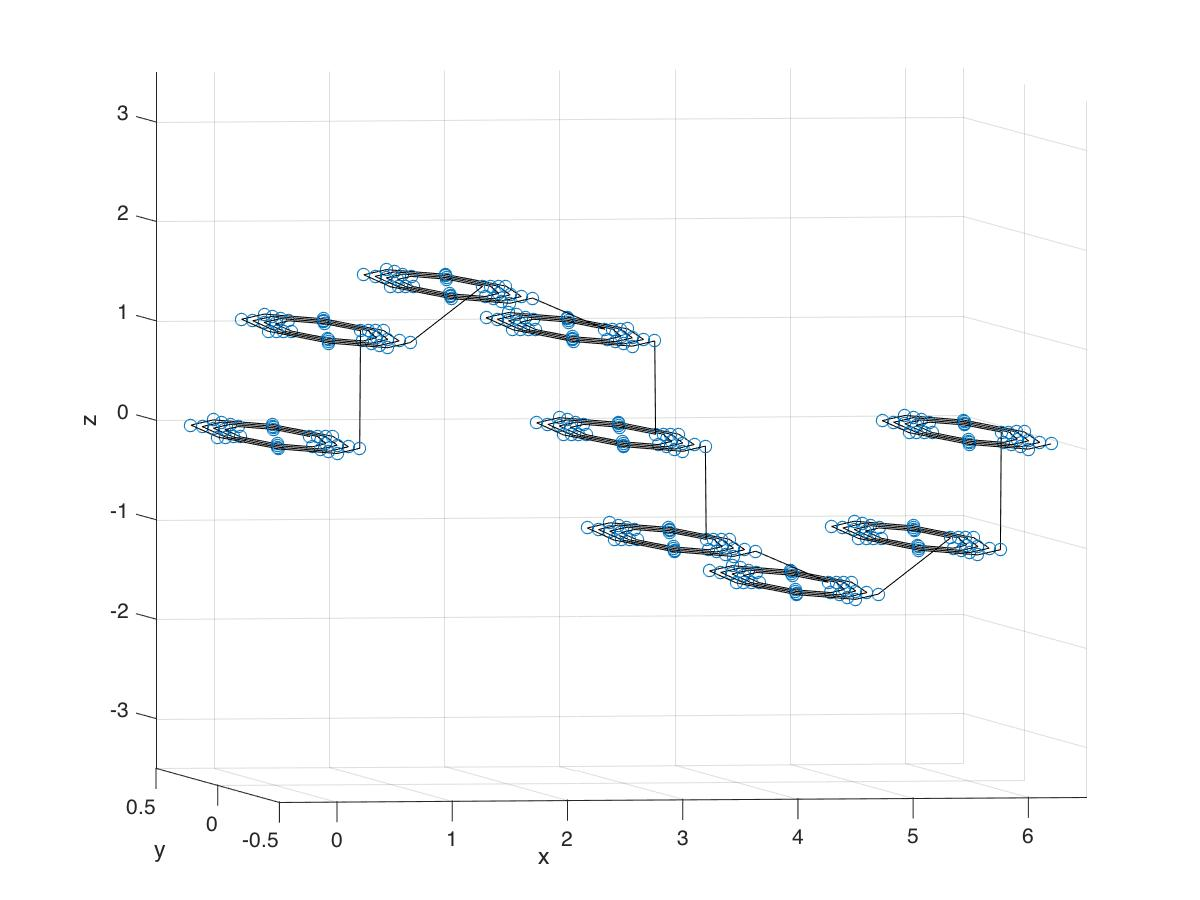
\includegraphics[width=10cm]{NoTilt.jpg}
  \caption{Mesh for \(N_c=8, N_\theta=8, N_t=3\) with no tilt to the slices. Lines connect each coordinate for better visuality.}
\end{figure}
\end{comment}
The next step is to rotate the slices appropriately through the angle \(\Theta\) for each slice so that a tubular structure is formed. Only the \(x\) and \(z\) coordinates must be modified. To perform the tilt, the following quantities are computed using trigonometry:

\begin{equation}
\begin{aligned}
w=\sin{(\pi/2-\Theta)}(r+dt)\cos{(\theta)}/\sin{(pi/2)}\\
h = w\sin{(\Theta)}\\
p = w\cos{(\Theta)}\\
\end{aligned}
\end{equation}

To tilt the z-coordinate, for points in the first and fourth quadrant of each slice:

\begin{equation}
z_{new} = z - (-1)^{tube}h
\end{equation}

And for points in the second and third quadrant of each slice:

\begin{equation}
z_{new} = z + (-1)^{tube}h
\end{equation}

where \(tube\) is a variable indicating whether or not the slice is in the left or right half of the tube. For the left half of the tube, \(tube=1\), and in the right half, \(tube=2\).

\item Then, tilt the x-coordinates. For points in the first and fourth quadrants of each slice:

\begin{equation}
x_{new} = x + p
\end{equation}

And for points in the second and third quadrants of each slice:

\begin{equation}
x_{new} = x - p
\end{equation}

\item Finally, tilt the slices that exactly align with the peak and valley of the tube (for odd numbers of \(N_\theta\), this would not be performed). For the slices that align with the peaks and for nodes in the first and fourth quadrants, adjust the \(z\) coordinates according to:

\begin{equation}
z_{new} = z - (r+dt)\cos{(\theta)}
\end{equation}

And for points in the second and third quadrants:

\begin{equation}
z_{new} = z + (r+dt)\cos{(\theta)}
\end{equation}

The \(x\)-coordinates are adjusted by simply setting all of them to the centroid coordinate for that slice. 
\end{enumerate}

This process is fairly complicated, and reveals why meshing software is so valuable. The process here is left fairly general that it can apply for any values of \(N_\theta, N_c, N_t\), but any slight change in the geometry completely invalidates the program. The final mesh for \(N_c=8, N_\theta=8, N_t=3\) is shown below. This mesh is shown because the requested mesh with only \(N_c=4\) is relatively difficult to perceive in a 3-D plot in Matlab, so the following plot better reveals the mesh. Lines are drawn between each coordinate.



The coarser mesh, for \(N_c=4, N_\theta=8, N_t=3\) is shown below, again with lines connecting each coordinate for better visibility.



The mesh in Fig. \ref{fig:CoarseMesh} is shown below without the lines connecting each coordinate.



Note that this assignment did not provide the dimensions of the tube, so I assumed that the inner radius of each arch was 1, the radius of the inner hole of the tube 0.3, and the thickness of the tube 0.2.

\subsection{The Connectivity Matrix}

In order for this mesh to be useful for finite element implementation, a connectivity function must be defined to relate the local node numbering to the global node numbering. The mesh generated numbers the global nodes according to the order in which they were generated. For instance, the first 8 nodes are in the inner layer of the first slice, the next 8 are in the second layer of the first slice, and so on for the first slice. Then, moving to the next \(\Theta\) slice, the node numbering again begins on the inside of the tube and moves counterclockwise in layers until reaching the outside of the tube. This is shown schematically in the figures above by the black lines connecting the coordinates \textit{in the order in which the coordinates are generated}.

The connectivity matrix is an \(N\times8\) matrix, where \(N\) is the total number of elements and 8 is the number of local nodes per element (linear elements are assumed). The local node numbering is performed according to a clockwise fashion. The following schematic shows the node numbering, where the left portion shows the front face, and the right portion shows the back face, all while looking at the front face (i.e. the back face is not written with the perspective of looking at the outward-facing portion of the back face).

\begin{equation}
\begin{aligned}
4 -- 3 & \quad\quad & 8 -- 7\\
2 -- 1 & \quad\quad & 6 -- 5\\
\end{aligned}
\end{equation}

So, for each slice, the nodes on the face of each element can be determined using a numbering scheme that follows the order in which the nodes were defined. Beginning with \(\theta=0\), and moving counterclockwise, the local nodes are numbered, moving progressively outwards in the layers until reaching the last node for a particular slice. 

There are \(N_t\cdot N_c\cdot N_\theta\) total elements. For each slice, the nodes are numbered moving counterclockwise, beginning at the same node that is meshed first. After each layer is complete, the numbering moves to the next layer in the same fashion. Once an entire slice is complete, the next slice is also meshed. This defines only the \textit{frontal} node numberings shown in the above equation. For example, for \(N_\theta=2, N_t=3, N_c=4\), the connectivity matrix \(\textbf{LM}\) looks like the following \textit{before} the nodes on the backs of the first 12 elements are related to the nodes on the fronts of the next 12 elements.

\begin{equation}
\textbf{LM}=
\begin{bmatrix}
1 & 2 & 5 & 6 & 0 & 0 & 0 & 0\\
2 & 3 & 6 & 7 & 0 & 0 & 0 & 0\\
3 & 4 & 7 & 8 & 0 & 0 & 0 & 0\\
4 & 1 & 8 & 5 & 0 & 0 & 0 & 0\\
5 & 6 & 9 & 10 & 0 & 0 & 0 & 0\\
6 & 7 & 10 & 11 & 0 & 0 & 0 & 0\\
7 & 8 & 11 & 12 & 0 & 0 & 0 & 0\\
8 & 5 & 12 & 9 & 0 & 0 & 0 & 0\\
9 & 10 & 13 & 14 & 0 & 0 & 0 & 0\\
10 & 11 & 14 & 15 & 0 & 0 & 0 & 0\\
11 & 12 & 15 & 16 & 0 & 0 & 0 & 0\\
12 & 9 & 16 & 13 & 0 & 0 & 0 & 0\\
17 & 18 & 21 & 22 & 0 & 0 & 0 & 0\\
18 & 19 & 22 & 23 & 0 & 0 & 0 & 0\\
19 & 20 & 23 & 24 & 0 & 0 & 0 & 0\\
20 & 17 & 24 & 21 & 0 & 0 & 0 & 0\\
21 & 22 & 25 & 26 & 0 & 0 & 0 & 0\\
22 & 23 & 26 & 27 & 0 & 0 & 0 & 0\\
23 & 24 & 27 & 28 & 0 & 0 & 0 & 0\\
24 & 21 & 28 & 25 & 0 & 0 & 0 & 0\\
25 & 26 & 29 & 30 & 0 & 0 & 0 & 0\\
26 & 27 & 30 & 31 & 0 & 0 & 0 & 0\\
27 & 28 & 31 & 32 & 0 & 0 & 0 & 0\\
28 & 25 & 32 & 29 & 0 & 0 & 0 & 0\\
33 & 34 & 37 & 38 & 0 & 0 & 0 & 0\\
34 & 35 & 38 & 39 & 0 & 0 & 0 & 0\\
35 & 36 & 39 & 40 & 0 & 0 & 0 & 0\\
36 & 33 & 40 & 37 & 0 & 0 & 0 & 0\\
37 & 38 & 41 & 42 & 0 & 0 & 0 & 0\\
38 & 39 & 42 & 43 & 0 & 0 & 0 & 0\\
39 & 40 & 43 & 44 & 0 & 0 & 0 & 0\\
40 & 37 & 44 & 41 & 0 & 0 & 0 & 0\\
41 & 42 & 45 & 46 & 0 & 0 & 0 & 0\\
42 & 43 & 46 & 47 & 0 & 0 & 0 & 0\\
43 & 44 & 47 & 48 & 0 & 0 & 0 & 0\\
44 & 41 & 48 & 45 & 0 & 0 & 0 & 0\\
\end{bmatrix}
\end{equation}

This is not the final form for the connectivity matrix (a.k.a. location matrix). Because the slices lay exactly on top of one another, the front nodes of the second slice are exactly the back nodes on the previous slice. With this knowledge, the back nodes for each element can be assigned based on the frontal nodes of the following slice. Then, the last \(N_cN_t\) rows in the location matrix above can be deleted, since they refer to the frontal nodes of a slice that does not technically exist (there are only 2 slices, but 3 planes defining those slices). With this information, the final form of the location matrix becomes, for \(N_\theta=2, N_t=3, N_c=4\) for example:

\begin{equation}
\textbf{LM}=
\begin{bmatrix}
1 & 2 & 5 & 6 & 17 & 18 & 21 & 22\\
2 & 3 & 6 & 7 & 18 & 19 & 22 & 23\\
3 & 4 & 7 & 8 & 19 & 20 & 23 & 24\\
4 & 1 & 8 & 5 & 20 & 17 & 24 & 21\\
5 & 6 & 9 & 10 & 21 & 22 & 25 & 26\\
6 & 7 & 10 & 11 & 22 & 23 & 26 & 27\\
7 & 8 & 11 & 12 & 23 & 24 & 27 & 28\\
8 & 5 & 12 & 9 & 24 & 21 & 28 & 25\\
9 & 10 & 13 & 14 & 25 & 26 & 29 & 30\\
10 & 11 & 14 & 15 & 26 & 27 & 30 & 31\\
11 & 12 & 15 & 16 & 27 & 28 & 31 & 32\\
12 & 9 & 16 & 13 & 28 & 25 & 32 & 29\\
17 & 18 & 21 & 22 & 33 & 34 & 37 & 38\\
18 & 19 & 22 & 23 & 34 & 35 & 38 & 39\\
19 & 20 & 23 & 24 & 35 & 36 & 39 & 40\\
20 & 17 & 24 & 21 & 36 & 33 & 40 & 37\\
21 & 22 & 25 & 26 & 37 & 38 & 41 & 42\\
22 & 23 & 26 & 27 & 38 & 39 & 42 & 43\\
23 & 24 & 27 & 28 & 39 & 40 & 43 & 44\\
24 & 21 & 28 & 25 & 40 & 37 & 44 & 41\\
25 & 26 & 29 & 30 & 41 & 42 & 45 & 46\\
26 & 27 & 30 & 31 & 42 & 43 & 46 & 47\\
27 & 28 & 31 & 32 & 43 & 44 & 47 & 48\\
28 & 25 & 32 & 29 & 44 & 41 & 48 & 45\\
\end{bmatrix}
\end{equation}

Each row in the location matrix corresponds to an elements, and each column to a local node number, so that \(LM(1,4)\) indicates the global node number of local node number 4 in element 1. This method is extended to the case for \(N_\theta=8, N_c=4, N_t=3\), where the purpose of the previous discussion for a fewer number of circumferential elements was simply to illustrate the process by which the location matrix is generated. So, for the problem statement in this homework assignment (\(N_\theta=8, N_c=4, N_t=3\)):

\begin{equation}
\label{eq:LMFinalForm}
\textbf{LM}=
\begin{bmatrix}LM_1 \\ LM_2\end{bmatrix}
\end{equation}

where, in order to be able to print the matrix, the following components are defined to simply be stacked on top of each other as in Eq. \eqref{eq:LMFinalForm}.

\begin{equation}
LM_1=
\begin{bmatrix}
1 & 2 & 5 & 6 & 17 & 18 & 21 & 22\\
2 & 3 & 6 & 7 & 18 & 19 & 22 & 23\\
3 & 4 & 7 & 8 & 19 & 20 & 23 & 24\\
4 & 1 & 8 & 5 & 20 & 17 & 24 & 21\\
5 & 6 & 9 & 10 & 21 & 22 & 25 & 26\\
6 & 7 & 10 & 11 & 22 & 23 & 26 & 27\\
7 & 8 & 11 & 12 & 23 & 24 & 27 & 28\\
8 & 5 & 12 & 9 & 24 & 21 & 28 & 25\\
9 & 10 & 13 & 14 & 25 & 26 & 29 & 30\\
10 & 11 & 14 & 15 & 26 & 27 & 30 & 31\\
11 & 12 & 15 & 16 & 27 & 28 & 31 & 32\\
12 & 9 & 16 & 13 & 28 & 25 & 32 & 29\\
17 & 18 & 21 & 22 & 33 & 34 & 37 & 38\\
18 & 19 & 22 & 23 & 34 & 35 & 38 & 39\\
19 & 20 & 23 & 24 & 35 & 36 & 39 & 40\\
20 & 17 & 24 & 21 & 36 & 33 & 40 & 37\\
21 & 22 & 25 & 26 & 37 & 38 & 41 & 42\\
22 & 23 & 26 & 27 & 38 & 39 & 42 & 43\\
23 & 24 & 27 & 28 & 39 & 40 & 43 & 44\\
24 & 21 & 28 & 25 & 40 & 37 & 44 & 41\\
25 & 26 & 29 & 30 & 41 & 42 & 45 & 46\\
26 & 27 & 30 & 31 & 42 & 43 & 46 & 47\\
27 & 28 & 31 & 32 & 43 & 44 & 47 & 48\\
28 & 25 & 32 & 29 & 44 & 41 & 48 & 45\\
33 & 34 & 37 & 38 & 49 & 50 & 53 & 54\\
34 & 35 & 38 & 39 & 50 & 51 & 54 & 55\\
35 & 36 & 39 & 40 & 51 & 52 & 55 & 56\\
36 & 33 & 40 & 37 & 52 & 49 & 56 & 53\\
37 & 38 & 41 & 42 & 53 & 54 & 57 & 58\\
38 & 39 & 42 & 43 & 54 & 55 & 58 & 59\\
39 & 40 & 43 & 44 & 55 & 56 & 59 & 60\\
40 & 37 & 44 & 41 & 56 & 53 & 60 & 57\\
41 & 42 & 45 & 46 & 57 & 58 & 61 & 62\\
42 & 43 & 46 & 47 & 58 & 59 & 62 & 63\\
43 & 44 & 47 & 48 & 59 & 60 & 63 & 64\\
44 & 41 & 48 & 45 & 60 & 57 & 64 & 61\\
49 & 50 & 53 & 54 & 65 & 66 & 69 & 70\\
50 & 51 & 54 & 55 & 66 & 67 & 70 & 71\\
51 & 52 & 55 & 56 & 67 & 68 & 71 & 72\\
52 & 49 & 56 & 53 & 68 & 65 & 72 & 69\\
53 & 54 & 57 & 58 & 69 & 70 & 73 & 74\\
54 & 55 & 58 & 59 & 70 & 71 & 74 & 75\\
55 & 56 & 59 & 60 & 71 & 72 & 75 & 76\\
56 & 53 & 60 & 57 & 72 & 69 & 76 & 73\\
57 & 58 & 61 & 62 & 73 & 74 & 77 & 78\\
58 & 59 & 62 & 63 & 74 & 75 & 78 & 79\\
59 & 60 & 63 & 64 & 75 & 76 & 79 & 80\\
60 & 57 & 64 & 61 & 76 & 73 & 80 & 77\\
65 & 66 & 69 & 70 & 81 & 82 & 85 & 86\\
\end{bmatrix}
\end{equation}

\begin{equation}
LM_2=
\begin{bmatrix}
66 & 67 & 70 & 71 & 82 & 83 & 86 & 87\\
67 & 68 & 71 & 72 & 83 & 84 & 87 & 88\\
68 & 65 & 72 & 69 & 84 & 81 & 88 & 85\\
69 & 70 & 73 & 74 & 85 & 86 & 89 & 90\\
70 & 71 & 74 & 75 & 86 & 87 & 90 & 91\\
71 & 72 & 75 & 76 & 87 & 88 & 91 & 92\\
72 & 69 & 76 & 73 & 88 & 85 & 92 & 89\\
73 & 74 & 77 & 78 & 89 & 90 & 93 & 94\\
74 & 75 & 78 & 79 & 90 & 91 & 94 & 95\\
75 & 76 & 79 & 80 & 91 & 92 & 95 & 96\\
76 & 73 & 80 & 77 & 92 & 89 & 96 & 93\\
81 & 82 & 85 & 86 & 97 & 98 & 101 & 102\\
82 & 83 & 86 & 87 & 98 & 99 & 102 & 103\\
83 & 84 & 87 & 88 & 99 & 100 & 103 & 104\\
84 & 81 & 88 & 85 & 100 & 97 & 104 & 101\\
85 & 86 & 89 & 90 & 101 & 102 & 105 & 106\\
86 & 87 & 90 & 91 & 102 & 103 & 106 & 107\\
87 & 88 & 91 & 92 & 103 & 104 & 107 & 108\\
88 & 85 & 92 & 89 & 104 & 101 & 108 & 105\\
89 & 90 & 93 & 94 & 105 & 106 & 109 & 110\\
90 & 91 & 94 & 95 & 106 & 107 & 110 & 111\\
91 & 92 & 95 & 96 & 107 & 108 & 111 & 112\\
92 & 89 & 96 & 93 & 108 & 105 & 112 & 109\\
97 & 98 & 101 & 102 & 113 & 114 & 117 & 118\\
98 & 99 & 102 & 103 & 114 & 115 & 118 & 119\\
99 & 100 & 103 & 104 & 115 & 116 & 119 & 120\\
100 & 97 & 104 & 101 & 116 & 113 & 120 & 117\\
101 & 102 & 105 & 106 & 117 & 118 & 121 & 122\\
102 & 103 & 106 & 107 & 118 & 119 & 122 & 123\\
103 & 104 & 107 & 108 & 119 & 120 & 123 & 124\\
104 & 101 & 108 & 105 & 120 & 117 & 124 & 121\\
105 & 106 & 109 & 110 & 121 & 122 & 125 & 126\\
106 & 107 & 110 & 111 & 122 & 123 & 126 & 127\\
107 & 108 & 111 & 112 & 123 & 124 & 127 & 128\\
108 & 105 & 112 & 109 & 124 & 121 & 128 & 125\\
113 & 114 & 117 & 118 & 129 & 130 & 133 & 134\\
114 & 115 & 118 & 119 & 130 & 131 & 134 & 135\\
115 & 116 & 119 & 120 & 131 & 132 & 135 & 136\\
116 & 113 & 120 & 117 & 132 & 129 & 136 & 133\\
117 & 118 & 121 & 122 & 133 & 134 & 137 & 138\\
118 & 119 & 122 & 123 & 134 & 135 & 138 & 139\\
119 & 120 & 123 & 124 & 135 & 136 & 139 & 140\\
120 & 117 & 124 & 121 & 136 & 133 & 140 & 137\\
121 & 122 & 125 & 126 & 137 & 138 & 141 & 142\\
122 & 123 & 126 & 127 & 138 & 139 & 142 & 143\\
123 & 124 & 127 & 128 & 139 & 140 & 143 & 144\\
124 & 121 & 128 & 125 & 140 & 137 & 144 & 141\\
\end{bmatrix}
\end{equation}

\subsection{Mesh Quality}

In order for the integrals in the weak form to remain finite when transformed to the master element, the Jacobian of the transformation must be positive. For a 3-D implementation, this means that \(\mathscr{J}\equiv\det{(\textbf{F})}>0\). A mesh has poor quality if it has elements with negative or zero Jacobians. This can occur for nonconvex elements, where some region of the master domain is mapped outside of the element when transforming back to the physical domain, or when the node numbering is performed incorrectly within an element such that the element is mapped inside-out. The Jacobian is not necessarily constant over an element, and it is required that the Jacobian be positive everywhere in the element - if the Jacobian were allowed to be negative over some regions of the element, but positive over others, this could cause singularities in the stiffness matrix.

\section{Computational Cost}

The cost of a 3-D finite element simulation of a vector-valued equation such as the equation of linear elasticity results in element stiffness matrices of size \(24\times24\) when using trilinear shape functions. For a cubical mesh, with \(M\times M\) elements, there are \(3(M+1)^3\) total unknowns in the mesh, so the global stiffness matrix is of size \((3(M+1)^3)\times(3(M+1)^3)\). If the symmetry of the local stiffness matrices is taken into account (they will always be symmetric for linear differential equations so long as the Bubnov-Galerkin approach is used), then the required storage per element drops from 576 to 300. 

If the Conjugate Gradient (CG) method is used to solve the matrix system \(\textbf{K}\textbf{a}=\textbf{R}\), then this represents repeated application of a \(24\times24\) matrix and a \(24\times1\) vector, which is an \(\mathscr{O}(N)\) operation. This is performed for each iteration, so the cost for the CG method scales as \(\mathscr{O}(IN)\), where \(I\) is the number of iterations needed to reach a particular tolerance in the solve.

The cost of a solve refers to both the storage required and the number of floating point operations required. There are three ways to perform the storage for a mesh consisting of \(M\times M\times M\) linear elements:

\begin{enumerate}
\item Direct storage - all zeros are stored, and no shortcuts are made by saving element-by-element. This requires \((3(M+1)^3)\times(3(M+1)^3)\approx9M^6\)
\item Element-by-element storage: no zeros are stored. This requires \(24\times24\times M^3=576M^3\)
\item Element-by-element storage, taking advantage of the symmetry of the element stiffness matrices. This requires \(300M^3\)
\end{enumerate} 

So, the storage scales cubically when using element-by-element storage as opposed to direct storage. The number of floating point operations is significantly reduced when using an iterative solver. The total number of unknowns is \(3(M+1)^3\), so the ratio of the direct solver (Gaussian elimination) to the CG method is:

\begin{equation}
\frac{\mathscr{O}(N^3)}{I\mathscr{O}(N)}=\frac{\left(3(M+1)^3\right)^2}{I}=\frac{9(M+1)^6}{I}
\end{equation}

where \(N=3(M+1)^3\) is the total number of unknowns. For \(N_t\times N_c\times N_\theta\) elements, there are \((N_t+1)N_c(N_\theta+1)\) total nodes. So, if there are 3 unknowns per node, and if a CG solver takes \(I\mathscr{O}(N)\) operations, then the total number of operations required is:

\begin{equation}
\text{Operations with CG method}=3I(N_t+1)N_c(N_\theta+1)
\end{equation}
 
 where \(I\) is the number of iterations.

\section{Appendix}

This section contains the complete code used in this assignment. 
\begin{comment}
\subsection{\texttt{MeshGenerator.m}}
This program generates the mesh and connectivity matrix.
\lstinputlisting[language=Matlab]{MeshGenerator.m}
\end{comment}

\end{document}